\documentclass[onecolumn]{IEEEtran}

\usepackage{pgfplots}
\usepackage{tikz}
\usetikzlibrary{arrows,shapes,decorations,backgrounds}

\begin{document}

\begin{figure}
  \centering
  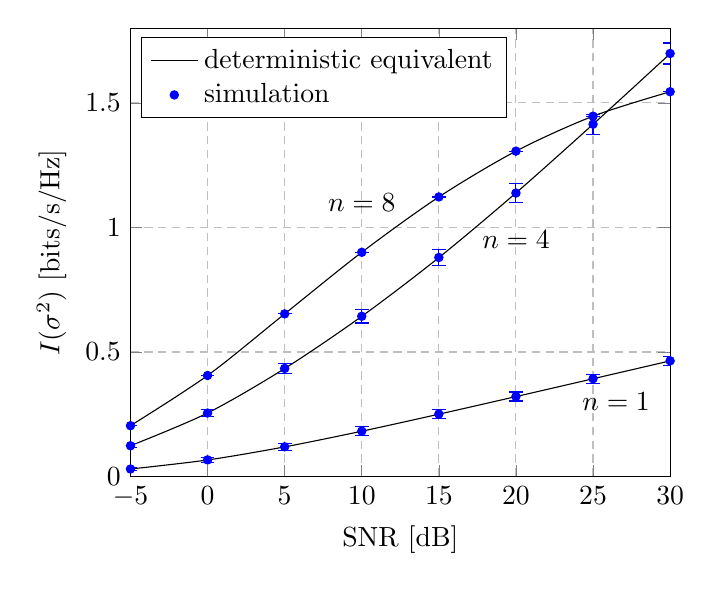
\begin{tikzpicture}
    \renewcommand{\axisdefaulttryminticks}{4}
    \pgfplotsset{every major grid/.append style={densely dashed}}
    \pgfplotsset{every axis legend/.append style={cells={anchor=west},fill=white, at={(0.02,0.98)}, anchor=north west}}
    \begin{axis}[
      xmin=-5,
      ymin=0,
      xmax=30,
      ymax=1.8,
      %xtick={-1,-0.3333,-0.2,0},
      %ytick={1,3,5},
      %xticklabels = {$-1$,$-\frac13$,$-\frac1{5}$,$0$},
      grid=major,
      %ymajorgrids=false,
      scaled ticks=true,
      %scale ticks above={4},
      ylabel={$I(\sigma^2)$ [bits/s/Hz]},
      xlabel={{\rm SNR} [dB]}
      ]
      \addplot[black,smooth] plot coordinates{
      (-5,0.030297) (0,0.066540) (5,0.119120) (10,0.182050) (15,0.250374) (20,0.321045) (25,0.392577) (30,0.464397) 
      };

      \addplot[blue,only marks,mark=*,mark options={scale=0.75},error bars/.cd,y dir=both,y explicit, error bar style={mark size=2.5pt}] plot coordinates{
      (-5,0.030333) +-(0.006501,0.006501) (0,0.066791) +-(0.011012,0.011012) (5,0.119404) +-(0.014716,0.014716) (10,0.182380) +-(0.017007,0.017007) (15,0.250934) +-(0.017914,0.017914) (20,0.321485) +-(0.018012,0.018012) (25,0.392825) +-(0.018163,0.018163) (30,0.464781) +-(0.018251,0.018251) 
      };

      \addplot[black,smooth] plot coordinates{
      (-5,0.123635) (0,0.255115) (5,0.433663) (10,0.643309) (15,0.879068) (20,1.138599) (25,1.414302) (30,1.697749) 
};

      \addplot[blue,only marks,mark=*,mark options={scale=0.75},error bars/.cd,y dir=both,y explicit, error bar style={mark size=2.5pt}] plot coordinates{
      (-5,0.123634) +-(0.008375,0.008375) (0,0.255066) +-(0.014449,0.014449) (5,0.434021) +-(0.020492,0.020492) (10,0.643461) +-(0.026844,0.026844) (15,0.879569) +-(0.032923,0.032923) (20,1.138196) +-(0.037653,0.037653) (25,1.414829) +-(0.040537,0.040537) (30,1.698557) +-(0.042252,0.042252) 
};

      \addplot[black,smooth] plot coordinates{
      (-5,0.204115) (0,0.405681) (5,0.653104) (10,0.900385) (15,1.122539) (20,1.306486) (25,1.446863) (30,1.545036) 
};

      \addplot[blue,only marks,mark=*,mark options={scale=0.75},error bars/.cd,y dir=both,y explicit, error bar style={mark size=2.5pt}] plot coordinates{
      (-5,0.204115) +-(0.000000,0.000000) (0,0.405681) +-(0.000000,0.000000) (5,0.653104) +-(0.000000,0.000000) (10,0.900385) +-(0.000000,0.000000) (15,1.122539) +-(0.000000,0.000000) (20,1.306486) +-(0.000000,0.000000) (25,1.446863) +-(0.000000,0.000000) (30,1.545036) +-(0.000000,0.000000) 
};

{\small
\node[] at (axis cs:10,1.1) {$n=8$}; 
\node[] at (axis cs:20,0.95) {$n=4$}; 
\node[] at (axis cs:26.5,0.3) {$n=1$}; 
}
      \legend{{deterministic equivalent},{simulation}}
    \end{axis}
  \end{tikzpicture}
  \caption{Mutual information $I(\sigma^2)$ versus ${\rm SNR}$ for different numbers of transmit signatures $n$, $N=16$, $N_i=8$, ${\bf P}_i={\bf I}_n$, $\alpha=0.5$. Error bars represent one standard deviation on each side.}
  \label{fig:mutual_info}
\end{figure}

%%%%%%%%%%%%%%%%%%%%%%


\begin{figure}
\centering
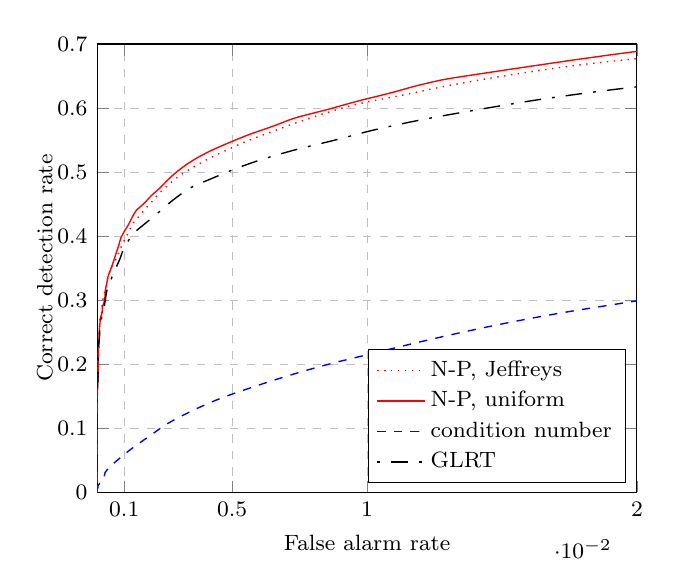
\begin{tikzpicture}[font=\footnotesize,scale=1]
\renewcommand{\axisdefaulttryminticks}{8}
\pgfplotsset{every major grid/.append style={dashed}}
\pgfplotsset{every axis legend/.append style={fill=white,cells={anchor=west},at={(0.98,0.02)},anchor=south east}}
\tikzstyle{dashed dotted}=[dash pattern=on 1pt off 4pt on 6pt off 4pt]

\begin{axis}[xlabel=False alarm rate,ylabel=Correct detection rate
,grid=major,
xmin=0,xmax=0.02,ymin=0.0,ymax=0.7,xtick={0.001,0.005,0.01,0.02},ylabel style={yshift=-5pt},
]

\addplot[smooth,red,dotted,line width=.5pt] plot coordinates {
(0.024550,0.696530) (0.020980,0.681530) (0.017710,0.666550) (0.015170,0.650860) (0.013110,0.635870) (0.011370,0.620740) (0.009710,0.606870) (0.008490,0.592620) (0.007430,0.577770) (0.006490,0.563290) (0.005560,0.548730) (0.004800,0.534470) (0.004130,0.521000) (0.003580,0.508260) (0.003060,0.494750) (0.002660,0.481040) (0.002320,0.467890) (0.002050,0.455110) (0.001780,0.442620) (0.001530,0.430110) (0.001290,0.417960) (0.001170,0.406060) (0.001010,0.394300) (0.000880,0.382580) (0.000770,0.370940) (0.000640,0.359580) (0.000500,0.348360) (0.000410,0.337700) (0.000360,0.327460) (0.000310,0.316790) (0.000230,0.305860) (0.000190,0.295710) (0.000170,0.285840) (0.000150,0.276790) (0.000090,0.268030) (0.000090,0.259330) (0.000080,0.250430) (0.000070,0.241370) (0.000060,0.232570) (0.000060,0.224490) (0.000040,0.216260) (0.000030,0.208760) (0.000030,0.201510) (0.000030,0.194340) (0.000030,0.187070) (0.000020,0.179730) (0.000020,0.173050) (0.000020,0.167020) (0.000010,0.160310) (0.000010,0.154020) (0.000010,0.147980) (0.000010,0.142120) (0.000010,0.136550) (0.000010,0.131170) (0,0.125890) (0,0.120420) (0,0.115390) (0,0.110690) (0,0.106130) (0,0.101670) (0,0.097520) (0,0.093240) (0,0.089420) (0,0.085540) (0,0.082010) (0,0.078300) (0,0.074860) (0,0.071670) (0,0.068350) (0,0.065440) (0,0.062750) (0,0.060000) (0,0.057460) (0,0.054850) (0,0.052310) (0,0.049770) (0,0.047380) (0,0.045060) (0,0.042790) (0,0.040640) (0,0.038430) (0,0.036550) (0,0.034890) (0,0.033050) (0,0.031150) (0,0.029580) (0,0.027840) (0,0.026370) (0,0.025020) (0,0.023710) (0,0.022250) (0,0.020990) (0,0.019840) (0,0.018730) (0,0.017800) (0,0.016920) (0,0.015990) (0,0.015170) (0,0.014260) (0,0.013430) (0,0.012700) (0,0.012010) (0,0.011250) (0,0.010610) (0,0.009950) (0,0.009500) (0,0.008920) (0,0.008430) (0,0.007930) (0,0.007370) (0,0.006960) (0,0.006640) (0,0.006260) (0,0.005900) (0,0.005650) (0,0.005260) (0,0.004950) (0,0.004610) (0,0.004350) (0,0.004030) (0,0.003790) (0,0.003590) (0,0.003420) (0,0.003190) (0,0.002970) (0,0.002820) (0,0.002680) (0,0.002540) (0,0.002340) (0,0.002170) (0,0.002000) (0,0.001910) (0,0.001830) (0,0.001700) (0,0.001570) (0,0.001450) (0,0.001310) (0,0.001230) (0,0.001110) (0,0.001010) (0,0.000950) (0,0.000930) (0,0.000850) (0,0.000790) (0,0.000770) (0,0.000720) (0,0.000640) (0,0.000600) (0,0.000560) (0,0.000530) (0,0.000510) (0,0.000470) (0,0.000430) (0,0.000420) (0,0.000380) (0,0.000340) (0,0.000320) (0,0.000290) (0,0.000240) (0,0.000210) (0,0.000170) (0,0.000130) (0,0.000120) (0,0.000100) (0,0.000090) (0,0.000090) (0,0.000080) (0,0.000070) (0,0.000060) (0,0.000060) (0,0.000050) (0,0.000050) (0,0.000050) (0,0.000050) (0,0.000040) (0,0.000040) (0,0.000040) (0,0.000040) (0,0.000030) (0,0.000030) (0,0.000030) (0,0.000020) (0,0.000020) (0,0.000020) (0,0.000010) (0,0.000010) (0,0.000010) (0,0.000010) (0,0.000010) (0,0.000010) (0,0.000010) (0,0.000010) (0,0.000010) (0,0.000010) (0,0.000010) (0,0.000010) (0,0.000010) (0,0.000010) (0,0.000010) (0,0) 

};

\addplot[smooth,red,line width=.5pt] plot coordinates {
(0.024550,0.69) (0.020980,0.693) 
(0.013780,0.650930) (0.012080,0.637360) (0.010890,0.623860) (0.009650,0.610840) (0.008540,0.597870) (0.007340,0.584670) (0.006520,0.571830) (0.005630,0.558690) (0.004910,0.546450) (0.004240,0.534120) (0.003690,0.522020) (0.003250,0.510140) (0.002880,0.498150) (0.002580,0.486390) (0.002320,0.475110) (0.002010,0.463550) (0.001740,0.451430) (0.001440,0.439910) (0.001290,0.429080) (0.001160,0.418160) (0.001000,0.407420) (0.000870,0.396610) (0.000800,0.386060) (0.000720,0.376170) (0.000640,0.365610) (0.000560,0.355510) (0.000470,0.345260) (0.000390,0.335650) (0.000350,0.325590) (0.000300,0.316200) (0.000290,0.306970) (0.000260,0.298120) (0.000190,0.289410) (0.000180,0.280850) (0.000120,0.272650) (0.000100,0.264430) (0.000080,0.256600) (0.000070,0.248460) (0.000070,0.240830) (0.000070,0.233650) (0.000050,0.226290) (0.000040,0.219200) (0.000040,0.211920) (0.000030,0.204820) (0.000030,0.197950) (0.000030,0.191180) (0.000030,0.184840) (0.000030,0.178760) (0.000010,0.172750) (0.000010,0.166740) (0.000010,0.161140) (0.000010,0.155650) (0,0.150370) (0,0.145030) (0,0.139940) (0,0.134990) (0,0.130000) (0,0.125630) (0,0.121280) (0,0.117070) (0,0.113280) (0,0.108990) (0,0.105260) (0,0.101190) (0,0.097210) (0,0.093780) (0,0.090480) (0,0.086870) (0,0.083490) (0,0.080240) (0,0.077500) (0,0.074440) (0,0.071660) (0,0.068990) (0,0.066310) (0,0.063460) (0,0.060910) (0,0.058280) (0,0.055780) (0,0.053530) (0,0.051220) (0,0.049060) (0,0.046800) (0,0.044730) (0,0.042660) (0,0.040720) (0,0.039150) (0,0.037650) (0,0.035980) (0,0.034530) (0,0.032880) (0,0.031690) (0,0.030060) (0,0.028710) (0,0.027410) (0,0.026070) (0,0.024920) (0,0.023710) (0,0.022740) (0,0.021780) (0,0.020800) (0,0.019800) (0,0.018750) (0,0.017930) (0,0.017130) (0,0.016420) (0,0.015720) (0,0.015030) (0,0.014310) (0,0.013640) (0,0.013050) (0,0.012300) (0,0.011730) (0,0.011030) (0,0.010390) (0,0.009880) (0,0.009360) (0,0.008930) (0,0.008560) (0,0.008100) (0,0.007690) (0,0.007250) (0,0.006900) (0,0.006490) (0,0.006190) (0,0.005830) (0,0.005560) (0,0.005170) (0,0.004900) (0,0.004580) (0,0.004320) (0,0.004100) (0,0.003760) (0,0.003520) (0,0.003280) (0,0.003140) (0,0.002980) (0,0.002760) (0,0.002600) (0,0.002440) (0,0.002300) (0,0.002200) (0,0.002070) (0,0.001930) (0,0.001820) (0,0.001700) (0,0.001610) (0,0.001520) (0,0.001330) (0,0.001240) (0,0.001140) (0,0.001060) (0,0.000960) (0,0.000920) (0,0.000880) (0,0.000810) (0,0.000730) (0,0.000670) (0,0.000640) (0,0.000610) (0,0.000550) (0,0.000510) (0,0.000490) (0,0.000460) (0,0.000430) (0,0.000400) (0,0.000400) (0,0.000380) (0,0.000340) (0,0.000300) (0,0.000270) (0,0.000250) (0,0.000200) (0,0.000190) (0,0.000180) (0,0.000180) (0,0.000160) (0,0.000160) (0,0.000140) (0,0.000130) (0,0.000100) (0,0.000100) (0,0.000090) (0,0.000080) (0,0.000080) (0,0.000070) (0,0.000060) (0,0.000060) (0,0.000050) (0,0.000040) (0,0.000040) (0,0.000020) (0,0.000020) (0,0.000020) (0,0.000020) (0,0.000020) (0,0.000020) (0,0.000020) (0,0.000010) (0,0) 
};

\addplot[smooth,blue,dashed,line width=.5pt] plot coordinates {
(0.999990,1.000000) (0.672840,0.955570) (0.248160,0.770960) (0.092870,0.566240) (0.039540,0.404260) (0.018470,0.288860) (0.009330,0.207980) (0.004970,0.152910) (0.002880,0.113810) (0.001870,0.085860) (0.001190,0.065510) (0.000750,0.050360) (0.000450,0.039010) (0.000290,0.030810) (0.000260,0.024550) (0.000190,0.019740) (0.000140,0.016260) (0.000070,0.012890) (0.000030,0.010630) (0.000020,0.008900) (0.000020,0.007250) (0.000010,0.006030) (0,0.005140) (0,0.004410) (0,0.003790) (0,0.003350) (0,0.002810) (0,0.002240) (0,0.001920) (0,0.001710) (0,0.001530) (0,0.001410) (0,0.001200) (0,0.001070) (0,0.000990) (0,0.000890) (0,0.000780) (0,0.000690) (0,0.000640) (0,0.000580) (0,0.000510) (0,0.000450) (0,0.000440) (0,0.000380) (0,0.000360) (0,0.000330) (0,0.000310) (0,0.000300) (0,0.000270) (0,0.000250) (0,0.000230) (0,0.000220) (0,0.000190) (0,0.000170) (0,0.000140) (0,0.000120) (0,0.000120) (0,0.000120) (0,0.000110) (0,0.000100) (0,0.000090) (0,0.000080) (0,0.000080) (0,0.000070) (0,0.000070) (0,0.000070) (0,0.000070) (0,0.000070) (0,0.000070) (0,0.000070) (0,0.000070) (0,0.000070) (0,0.000070) (0,0.000070) (0,0.000070) (0,0.000070) (0,0.000060) (0,0.000050) (0,0.000050) (0,0.000050) (0,0.000050) (0,0.000050) (0,0.000050) (0,0.000050) (0,0.000040) (0,0.000040) (0,0.000030) (0,0.000030) (0,0.000030) (0,0.000020) (0,0.000020) (0,0.000020) (0,0.000020) (0,0.000020) (0,0.000020) (0,0.000020) (0,0.000020) (0,0.000020) (0,0.000020) (0,0.000020) (0,0.000020) (0,0.000020) (0,0.000020) (0,0.000020) (0,0.000020) (0,0.000020) (0,0.000020) (0,0.000020) (0,0.000020) (0,0.000020) (0,0.000020) (0,0.000020) (0,0.000020) (0,0.000020) (0,0.000020) (0,0.000020) (0,0.000020) (0,0.000020) (0,0.000020) (0,0.000020) (0,0.000020) (0,0.000020) (0,0.000020) (0,0.000020) (0,0.000020) (0,0.000020) (0,0.000020) (0,0.000020) (0,0.000020) (0,0.000020) (0,0.000020) (0,0.000020) (0,0.000020) (0,0.000020) (0,0.000020) (0,0.000020) (0,0.000020) (0,0.000020) (0,0.000020) (0,0.000020) (0,0.000010) (0,0.000010) (0,0.000010) (0,0.000010) (0,0.000010) (0,0.000010) (0,0.000010) (0,0.000010) (0,0.000010) (0,0.000010) (0,0.000010) (0,0.000010) (0,0.000010) (0,0.000010) (0,0.000010) (0,0.000010) (0,0.000010) (0,0.000010) (0,0.000010) (0,0.000010) (0,0.000010) (0,0.000010) (0,0.000010) (0,0.000010) (0,0.000010) (0,0.000010) (0,0.000010) (0,0.000010) (0,0.000010) (0,0.000010) (0,0.000010) (0,0.000010) (0,0.000010) (0,0.000010) (0,0.000010) (0,0.000010) (0,0.000010) (0,0.000010) (0,0.000010) (0,0.000010) (0,0.000010) (0,0.000010) (0,0.000010) (0,0.000010) (0,0.000010) (0,0.000010) (0,0.000010) (0,0.000010) (0,0.000010) (0,0.000010) (0,0.000010) (0,0.000010) (0,0.000010) (0,0.000010) (0,0.000010) (0,0.000010) (0,0.000010) (0,0.000010) (0,0.000010) (0,0)
};

\addplot[smooth,black,dashed dotted,line width=.5pt] plot coordinates {
(0.999990,1.000000) (0.999840,1.000000) (0.999010,0.999940) (0.995530,0.999760) (0.986900,0.999270) (0.970660,0.998300) (0.945370,0.996530) (0.911750,0.994340) (0.868510,0.990770) (0.819520,0.986690) (0.763490,0.981090) (0.705600,0.974540) (0.646570,0.967040) (0.587180,0.958550) (0.529600,0.949080) (0.475600,0.938770) (0.423830,0.927670) (0.375280,0.916620) (0.330170,0.904620) (0.290120,0.891510) (0.253340,0.878360) (0.221150,0.864500) (0.191750,0.850420) (0.165190,0.835410) (0.142500,0.820480) (0.122210,0.805430) (0.104580,0.790180) (0.089480,0.774870) (0.076700,0.59050) (0.065540,0.743320) (0.055920,0.727440) (0.047330,0.711870) (0.040360,0.695740) (0.033710,0.679490) (0.027850,0.663290) (0.023100,0.646770) (0.019370,0.630110) (0.016490,0.613980) (0.014100,0.597470) (0.012000,0.581580) (0.010260,0.565850) (0.008830,0.550210) (0.007380,0.535300) (0.006120,0.520040) (0.005120,0.505220) (0.004270,0.490480) (0.003480,0.476080) (0.002960,0.461250) (0.002520,0.446430) (0.002150,0.432550) (0.001740,0.418560) (0.001370,0.405260) (0.001140,0.391970) (0.000960,0.378640) (0.000850,0.365600) (0.000710,0.352290) (0.000580,0.340200) (0.000470,0.327510) (0.000360,0.315460) (0.000310,0.303870) (0.000270,0.292820) (0.000210,0.281690) (0.000150,0.270910) (0.000090,0.260810) (0.000090,0.251030) (0.000080,0.241110) (0.000050,0.231780) (0.000040,0.222280) (0.000040,0.213120) (0.000030,0.203840) (0.000030,0.195100) (0.000030,0.187120) (0.000020,0.179150) (0.000020,0.171360) (0.000010,0.164330) (0,0.157110) (0,0.150150) (0,0.143560) (0,0.136880) (0,0.130620) (0,0.124950) (0,0.119170) (0,0.114100) (0,0.109300) (0,0.104040) (0,0.099230) (0,0.094310) (0,0.089750) (0,0.085820) (0,0.081780) (0,0.077860) (0,0.074220) (0,0.070450) (0,0.066760) (0,0.063310) (0,0.059920) (0,0.056670) (0,0.053510) (0,0.050830) (0,0.048080) (0,0.045390) (0,0.043160) (0,0.040940) (0,0.038600) (0,0.036210) (0,0.034190) (0,0.032210) (0,0.030480) (0,0.028860) (0,0.027230) (0,0.025920) (0,0.024420) (0,0.022950) (0,0.021340) (0,0.020080) (0,0.018840) (0,0.017820) (0,0.016790) (0,0.015910) (0,0.014990) (0,0.014150) (0,0.013350) (0,0.012400) (0,0.011730) (0,0.010930) (0,0.010320) (0,0.009710) (0,0.009130) (0,0.008520) (0,0.007990) (0,0.007430) (0,0.006870) (0,0.006300) (0,0.005860) (0,0.005480) (0,0.005080) (0,0.004770) (0,0.004320) (0,0.004040) (0,0.003820) (0,0.003590) (0,0.003360) (0,0.003060) (0,0.002780) (0,0.002590) (0,0.002440) (0,0.002250) (0,0.002070) (0,0.001930) (0,0.001780) (0,0.001570) (0,0.001400) (0,0.001290) (0,0.001200) (0,0.001090) (0,0.001010) (0,0.000910) (0,0.000840) (0,0.000790) (0,0.000740) (0,0.000670) (0,0.000610) (0,0.000540) (0,0.000490) (0,0.000450) (0,0.000410) (0,0.000350) (0,0.000310) (0,0.000290) (0,0.000230) (0,0.000180) (0,0.000170) (0,0.000170) (0,0.000170) (0,0.000140) (0,0.000130) (0,0.000120) (0,0.000100) (0,0.000090) (0,0.000080) (0,0.000080) (0,0.000040) (0,0.000020) (0,0.000020) (0,0.000020) (0,0.000020) (0,0.000020) (0,0.000010) (0,0.000010) (0,0.000010) (0,0.000010) (0,0.000010) (0,0.000010) (0,0.000010) (0,0.000010) (0,0.000010) (0,0.000010) (0,0.000010) (0,0.000010) (0,0)
};

\legend{N-P, Jeffreys \\ N-P, uniform \\ condition number \\ GLRT \\};
\end{axis}
\end{tikzpicture}
\caption{ROC curve for a priori unknown $\sigma^2$ of the Neyman-Pearson test (N-P), condition number method and GLRT, $N=4$, $M=8$, ${\sf SNR}=0~{\rm dB}$, ${\bf h}\sim\mathcal{CN}(0,{\bf I}_N)$. For the Neyman-Pearson test, both uniform and Jeffreys prior, with exponent $\beta=1$, are provided.}
\label{fig:unknownSNR}
\end{figure}


%%%%%%%%%%%%%%%%%%%%%%

\begin{figure}
  \centering
  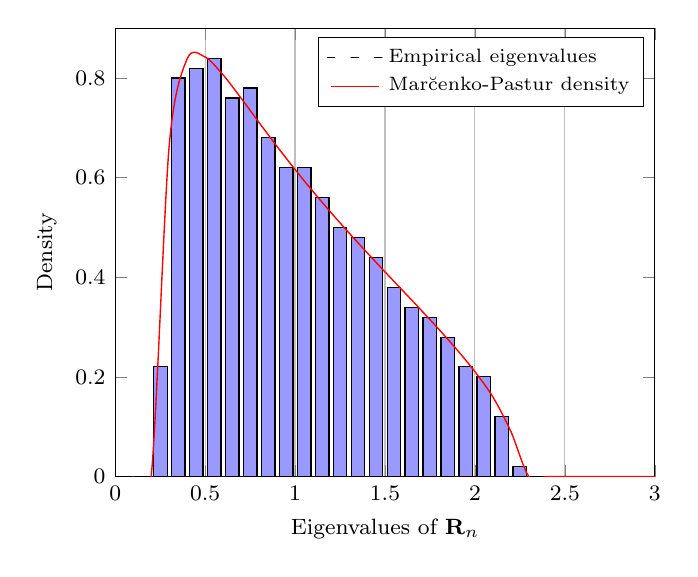
\begin{tikzpicture}[font=\footnotesize]
    \renewcommand{\axisdefaulttryminticks}{4} 
    %\pgfplotsset{every major grid/.append style={densely dashed}}       
    \pgfplotsset{every axis legend/.append style={cells={anchor=west},fill=white, at={(0.98,0.98)}, anchor=north east, font=\scriptsize }}
    \begin{axis}[
      %ybar,
      xmin=0,
      ymin=0,
      xmax=3,
      ymax=0.9,
      %xtick={0,1,2,3,4},
      ytick={0,0.2,0.4,0.6,0.8},
      yticklabels = {$0$,$0.2$,$0.4$,$0.6$,$0.8$},
      bar width=5pt,
      grid=major,
      ymajorgrids=false,
      scaled ticks=true,
      %scale ticks above={4},
      xlabel={Eigenvalues of ${\bf R}_n$},
      ylabel={Density}
      ]
      \addplot+[ybar,mark=none,color=black,fill=blue!40!white] coordinates{
      (0.050000,0.000000)(0.150000,0.000000)(0.250000,0.220000)(0.350000,0.800000)(0.450000,0.820000)(0.550000,0.840000)(0.650000,0.760000)(0.750000,0.780000)(0.850000,0.680000)(0.950000,0.620000)(1.050000,0.620000)(1.150000,0.560000)(1.250000,0.500000)(1.350000,0.480000)(1.450000,0.440000)(1.550000,0.380000)(1.650000,0.340000)(1.750000,0.320000)(1.850000,0.280000)(1.950000,0.220000)(2.050000,0.200000)(2.150000,0.120000)(2.250000,0.020000)(2.350000,0.000000)(2.450000,0.000000)(2.550000,0.000000)(2.650000,0.000000)(2.750000,0.000000)(2.850000,0.000000)(2.950000,0.000000)(3.050000,0.000000)(3.150000,0.000000)(3.250000,0.000000)(3.350000,0.000000)(3.450000,0.000000)(3.550000,0.000000)(3.650000,0.000000)(3.750000,0.000000)(3.850000,0.000000)(3.950000,0.000000)(4.050000,0.000000)(4.150000,0.000000)(4.250000,0.000000)(4.350000,0.000000)(4.450000,0.000000)(4.550000,0.000000)(4.650000,0.000000)(4.750000,0.000000)(4.850000,0.000000)(4.950000,0.000000)(5.050000,0.000000)
      };
      \addplot[smooth,red,line width=0.5pt] plot coordinates{
      (0.100000,0.000000)(0.200000,0.000000)(0.300000,0.662615)(0.400000,0.838401)(0.500000,0.842169)(0.600000,0.806315)(0.700000,0.759546)(0.800000,0.710650)(0.900000,0.662615)(1.000000,0.616404)(1.100000,0.572197)(1.200000,0.529853)(1.300000,0.489095)(1.400000,0.449584)(1.500000,0.410936)(1.600000,0.372721)(1.700000,0.334423)(1.800000,0.295379)(1.900000,0.254626)(2.000000,0.210542)(2.100000,0.159695)(2.200000,0.090357)(2.300000,0.000000)(2.400000,0.000000)(2.500000,0.000000)(2.600000,0.000000)(2.700000,0.000000)(2.800000,0.000000)(2.900000,0.000000)(3.000000,0.000000)
      };
      \legend{ {Empirical eigenvalues},{Mar\u{c}enko-Pastur density} }
    \end{axis}
  \end{tikzpicture}
  \caption{Histogram of the eigenvalues of ${\bf R}_n=\frac1n\sum_{k=1}^n{\bf x}_k{\bf x}_k^*$, ${\bf x}_k\sim \mathcal{CN}(0,{\bf I}_N)$, for $n=2000$, $N=500$.}
  \label{fig:empiricalMPlaw}
\end{figure}


%%%%%%%%%%%%%%%%%%%%%

\begin{figure}
\centering

\begin{tikzpicture}
\begin{axis}[
xlabel=$n_1$,
ylabel=$n_2$,
zlabel={\small Ergodic Sum-rate [bits/s/Hz]},
view/az=-36,
grid=major,
xtick={0,2,2,4,6,8,10},
ytick={0,2,4,6,8,10},
ztick={0,0.5,1,1.5,2},
zmin=0,
zmax=1.5,
legend style={at={(1.05,1.05)}, anchor={north east}}, font=\small]
\pgfplotsset{every major grid/.style={densely dotted}} 
\addlegendentry{{Simulation}};
\addlegendentry{{Approximation}};
\addlegendentry{{$(n_1^*,n_2^*)$}};

\addplot3[mesh,draw=black, line width=0.25] file {datasim0.txt};
\addplot3+[only marks,mark=+, mark size=2, mark options={color=black}] file {datadet0.txt};
\addplot3+[only marks,mark=x, mark size=4, mark options={color=red}, line width=1.5] coordinates {(10,10,1.111)};
\end{axis}
\end{tikzpicture}

\end{figure}

%%%%%%%%%%%%%%%%%%
%% my version of 
\begin{figure}
\centering

\begin{tikzpicture}
\begin{axis}[
xlabel=$f^{\prime}(\tau)$,
ylabel=$f^{\prime\prime}(\tau)$,
zlabel={\small Classification error},
%view/az=36,
view={60}{5},
grid=major,
xtick={-1,-0.5,0,0.5},
ytick={-0.5,0,0.5,1},
ztick={0,0.25,0.5,0.75},
legend style={at={(1.05,1.05)}, anchor={north east}}, font=\small]
\pgfplotsset{every major grid/.style={densely dotted}} 
\addlegendentry{{Theoretical error}};
\addlegendentry{{Real error}};
%\addlegendentry{{$(n_1^*,n_2^*)$}};

\addplot3[surf,draw=black, line width=0.25] file {data1.txt};
%\addplot3+[only marks,mark=x, mark size=2, mark options={color=black}] file {data2.txt};
% \addplot3+[only marks,mark=x, mark size=4, mark options={color=red}, line width=1.5] coordinates {(10,10,0.0530)};
% \addplot3+[only marks,mark=x, mark size=4, mark options={color=blue}, line width=1.5] coordinates {(10,10,0.0498)};

\end{axis}
\end{tikzpicture}

\end{figure}



%%%%%%%%%%%%%%%%%%


  \begin{figure}
    \centering

    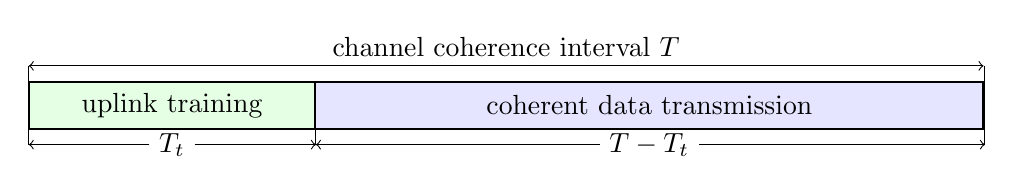
\begin{tikzpicture}

      % channel coherence interval
      \draw[black,thick,fill=black!10] (0,0) rectangle (\textwidth,0.6cm);
      \draw[black] (0,0.6cm) -- (0,0.8cm);
      \draw[black] (\textwidth+0.5pt,0.6cm) -- (\textwidth+0.5pt,0.8cm);
      \draw[black,<->] (0,0.8cm) -- node[midway,above] {channel coherence interval $T$} (\textwidth,0.8cm);

      % training
      \draw[black,thick,fill=green!10] (0,0) rectangle (.3\textwidth,0.6cm);
      \draw (.15\textwidth,0.3cm) node[draw=none] {uplink training};
      \draw[black] (0,0) -- (0,-0.2cm);
      \draw[black] (.3\textwidth+0.2pt,0) -- (.3\textwidth+0.2pt,-0.2cm);
      \draw (.15\textwidth,-.2cm) node[draw=none] (tr) {$T_t$};
      \draw[black,->] (tr) -- (0,-0.2cm);
      \draw[black,->] (tr) -- (.3\textwidth+0.25pt,-0.2cm);

      % data transmission
      \draw[black,thick,fill=blue!10] (.3\textwidth,0) rectangle (\textwidth,0.6cm);
      \draw (.65\textwidth,0.3cm) node[draw=none] {coherent data transmission};
      \draw[black] (\textwidth+0.5pt,0) -- (\textwidth+0.5pt,-.2cm);
      \draw (.65\textwidth,-.2cm) node[draw=none] (dt) {$T - T_t$};
      \draw[black,->] (dt) -- (\textwidth+0.5pt,-.2cm);
      \draw[black,->] (dt) -- (.3\textwidth+0.25pt,-0.2cm);
    
    \end{tikzpicture}
    
  \end{figure}

%%%%%%%%%%%%%%%%%%

\begin{figure}
	  \centering
  \def\w{1cm}
  \def\h{0.75cm}
  \def\ind{2cm} 
  \tikzstyle{block}=[rectangle,draw=black,thick,inner sep=0pt,minimum height=\h,minimum width=\w, rounded corners=0pt]
  \tikzstyle{connector}=[->,>=latex',semithick, double]
  \tikzstyle{connectorScalar}=[->,>=latex',semithick]
  \tikzstyle{adder}=[circle,draw=black,thick,inner sep=0pt,minimum size=1.5pt]
  \tikzstyle{antenna} = [draw=black,very thick,regular polygon,regular polygon sides=3,anchor=center]
  \tikzstyle{rxantenna} = [scale=0.5,draw=black,very thick,regular polygon,regular polygon sides=3,anchor=center]
  \tikzstyle{signalpath}=[draw,<->,>=latex',gray]
  \tikzstyle{every node}=[node distance=1.5cm,text centered]

  \begin{tikzpicture}

   % data symbols
   \node (s1) {$\bf s$};

    % power allocation
   \node[block] (p1) [right of=s1,text width=\w] {${\bf P}^{1/2}$};    

    
    % beamforming
    \node[block] (g1) [right of=p1, node distance=2cm,text width=\w] {$\bf G$};

    % sum
    \node[shape=circle=2pt,fill=black,inner sep=2pt] (dot) [right of=g1] {};    

    % tx antennas
    \node[antenna] (a2) [right of=dot,rotate=90,node distance=1.0cm] {};    
    \node[antenna] (a1) [above of=a2,rotate=90,node distance=1.0cm] {}; 
    \node[antenna] (aM) [below of=a2,rotate=90,node distance=1.0cm] {}; 


    \draw (s1) edge[connector]  (p1);
    \draw (p1) edge [connector] (g1);

    \draw (g1)  edge [connector] node[above] {$\bf x$} (dot);

    \draw[thick] (dot) -- node[above,pos=0.8] {$2$} (a2);
    \draw[thick] (dot) |- node[above,pos=0.9] {$1$} (a1);
    \draw[thick] (dot) |- node[above,pos=0.9] {$M$} (aM);

    % dots
    \draw (a2) edge[draw=none] node[midway,rotate=90] {\Large{...}} (aM);

    % user antennas
    \node[rxantenna] (u1a2) [right of=a1,rotate=-90,node distance=2.5cm] {};    
    \node[rxantenna] (u2a2) [right of=a2,rotate=-90,node distance=6cm] {};
    \node[rxantenna] (uKa2) [right of=aM,rotate=-90,node distance=2.5cm] {};    

    % user 1
    \node[adder] (u1sum) [right of=u1a2,node distance=1cm] {+};    
    \node (u1n) [below of=u1sum,node distance=0.6cm] {$n_1$};
    \node (u1rx) [right of=u1sum,node distance=1cm] {$y_1$};    

    \path (u1a2) edge [connectorScalar] (u1sum); 
    \path (u1n) edge [connectorScalar] (u1sum); 
    \path (u1sum) edge [connectorScalar] (u1rx);

    % user 2
    \node[adder] (u2sum) [right of=u2a2,node distance=1cm] {+};    
    \node (u2n) [above of=u2sum,node distance=0.6cm] {$n_2$};
    \node (u2rx) [right of=u2sum,node distance=1cm] {$y_2$};    

    \path (u2a2) edge [connectorScalar] (u2sum); 
    \path (u2sum) edge [connectorScalar] (u2rx);
    \path (u2n) edge [connectorScalar] (u2sum);  

    % user K
    \node[adder] (uKsum) [right of=uKa2,node distance=1cm] {+};        
    \node (uKn) [above of=uKsum,node distance=0.6cm] {$n_K$};
    \node (uKrx) [right of=uKsum,node distance=1cm] {$y_K$};    

    \path (uKa2) edge [connectorScalar] (uKsum); 
    \path (uKsum) edge [connectorScalar] (uKrx); 
    \path (uKn) edge [connectorScalar] (uKsum); 

    % channel
   \path
    (a1.south) edge[signalpath] (u1a2.south) 
    (a2.south) edge[signalpath] (u1a2.south) 
    (aM.south) edge[signalpath] (u1a2.south); 

   \draw (a1) edge[draw=none, bend left=30] node[midway] {$\mathbf{h}_1$} (u1a2);
    
   \path
    (a1.south) edge[signalpath] (u2a2.south) 
    (a2.south) edge[signalpath] (u2a2.south) 
    (aM.south) edge[signalpath] (u2a2.south); 

   \draw (a2) edge[draw=none, above] node[pos=0.4] {$\mathbf{h}_2$} (u2a2);

   \path
    (a1.south) edge[signalpath] (uKa2.south) 
    (a2.south) edge[signalpath] (uKa2.south) 
    (aM.south) edge[signalpath] (uKa2.south); 
   
   \draw (aM) edge[draw=none, bend right=30] node[midway] {$\mathbf{h}_K$} (uKa2);

    % dots
    \draw (u2sum) edge[draw=none] node[midway,rotate=90] {\Large{...}} (uKsum);

    % channel
    \tikzstyle{signalpath}=[draw=green!50,<->,>=latex',fill=green!50]

   \path
    (a1.south) edge[signalpath] (u1a2.south) 
    (a2.south) edge[signalpath] (u1a2.south) 
    (aM.south) edge[signalpath] (u1a2.south); 

   \path
    (a1.south) edge[signalpath] (u2a2.south) 
    (a2.south) edge[signalpath] (u2a2.south) 
    (aM.south) edge[signalpath] (u2a2.south); 

   \path
    (a1.south) edge[signalpath] (uKa2.south) 
    (a2.south) edge[signalpath] (uKa2.south) 
    (aM.south) edge[signalpath] (uKa2.south); 

    \node[adder,fill=green!50] (u1sum) [right of=u1a2,node distance=1cm] {+};    
    \node[adder,fill=green!50] (u2sum) [right of=u2a2,node distance=1cm] {+};  
    \node[adder,fill=green!50] (uKsum) [right of=uKa2,node distance=1cm] {+};        



  \end{tikzpicture}

\end{figure}

\end{document}
